\section{Chuyên Lê Khiết -- Quảng Ngãi - Lần 1. NH: 25-26}
%P1
\caulc
\setcounter{ex}{0}
\Opensolutionfile{ans}[ans/18-26-2-QuangNgai-ChuyenLeKhiet-L2_LC]
\begin{ex}
	 Cho hàm số $y = f(x)$ liên tục trên $\mathbb{R}$ và có một nguyên hàm là $F(x)$. Biết rằng $F(1) = 9$, $F(2) = 5$. Giá trị của biểu thức $\displaystyle\int\limits_{1}^{2} f(x) \mathrm{\,d}x$ bằng
	\choice
	{ $14$}
	{ \True $-4$}
	{ $45$}
	{ $4$}
	\loigiai{
		Ta có: $\displaystyle\int\limits_{1}^{2} f(x) \mathrm{\,d}x = F(2) - F(1) = 5 - 9 = -4$.
	}
\end{ex}

\begin{ex}
	 Tập nghiệm của bất phương trình $2^{2+x^2} > 16$ là
	\choice
	{ \True $\left(-\infty; -\sqrt{2}\right) \cup \left(\sqrt{2}; +\infty\right)$}
	{ $\left(-\infty; -\sqrt{2}\right] \cup \left[\sqrt{2}; +\infty\right)$}
	{ $(-\infty; -2) \cup (2; +\infty)$}
	{ $(-\infty; -2] \cup [2; +\infty)$}
	\loigiai{
		Ta có: $2^{2+x^2} > 16 \Leftrightarrow 2^{2+x^2} > 2^4 \Leftrightarrow 2 + x^2 > 4 \Leftrightarrow x^2 > 2 \Leftrightarrow \left[\begin{aligned} &x > \sqrt{2} \\ &x < -\sqrt{2} \end{aligned}\right.$\\
		Vậy tập nghiệm của bất phương trình là $S = \left(-\infty; -\sqrt{2}\right) \cup \left(\sqrt{2}; +\infty\right)$.
	}
\end{ex}

\begin{ex}
	\immini{
	 Cho hàm số $y = f(x)$ xác định trên $\mathbb{R}$ và có bảng biến thiên như bảng dưới đây. Khẳng định nào sau đây đúng?
	\choice
	{ Hàm số đồng biến trên khoảng $(1;2)$}
	{ Hàm số đồng biến trên khoảng $(-5;4)$}
	{ \True Hàm số nghịch biến trên khoảng $(1;2)$}
	{ Hàm số nghịch biến trên khoảng $(-5;4)$}
	}{
		
\begin{tikzpicture}
			\tkzTabInit[nocadre=false, lgt=0.8, espcl=1.6] 
			{$x$ /0.7,$y'$ /0.7,$y$ /1.7}
			{$-\infty$,$1$,$2$,$+\infty$}
			\tkzTabLine{,+,0,-,0,+,} 
			\tkzTabVar{-/$-\infty$ ,+/ $5$, -/ $-4$ /, +/$+\infty$ /} 
		\end{tikzpicture}
	}
	\loigiai{
		Dựa vào bảng biến thiên, trên khoảng $(1;2)$ ta có $f'(x) < 0$ nên hàm số nghịch biến trên khoảng $(1;2)$.
	}
\end{ex}

\begin{ex}
	 Họ nguyên hàm của hàm số $f(x) = \sin x$ là
	\choice
	{ $\sin x + C$}
	{ \True $-\cos x + C$}
	{ $-\sin x + C$}
	{ $\cos x + C$}
	\loigiai{
		Theo công thức nguyên hàm cơ bản ta có: $\int \sin x \mathrm{\,d}x = -\cos x + C$.
	}
\end{ex}

\begin{ex}
	 Mỗi ngày bác Mạnh đều đi bộ rèn luyện sức khoẻ. Quãng đường đi bộ mỗi ngày của bác trong $20$ ngày được thống kê lại ở bảng sau
	\begin{center}
		\begin{tabular}{|c|c|c|c|c|c|}
			\hline
			Quãng đường ($\text{km}$) & $[2{,}7; 3{,}0)$ & $[3{,}0; 3{,}3)$ & $[3{,}3; 3{,}6)$ & $[3{,}6; 3{,}9)$ & $[3{,}9; 4{,}2)$ \\ \hline
			Số ngày & $3$ & $6$ & $5$ & $4$ & $2$ \\ \hline
		\end{tabular}
	\end{center}
	Phương sai của mẫu số liệu ghép nhóm là
	\choice
	{ $1{,}26$}
	{ $0{,}26$}
	{ $0{,}19$}
	{ \True $0{,}13$}
	\loigiai{
		Chọn giá trị đại diện cho các nhóm lần lượt là: $x_1 = 2{,}85$; $x_2 = 3{,}15$; $x_3 = 3{,}45$; $x_4 = 3{,}75$; $x_5 = 4{,}05$.\\
		Số ngày khảo sát là $n = 3 + 6 + 5 + 4 + 2 = 20$.\\
		Số trung bình của mẫu số liệu ghép nhóm là:\\
		$\bar{x} = \dfrac{3 \cdot 2{,}85 + 6 \cdot 3{,}15 + 5 \cdot 3{,}45 + 4 \cdot 3{,}75 + 2 \cdot 4{,}05}{20} = 3{,}39$ (km).\\
		Phương sai của mẫu số liệu ghép nhóm là:\\
		$s^2 = \dfrac{1}{20} \left[ 3 \cdot (2{,}85 - 3{,}39)^2 + 6 \cdot (3{,}15 - 3{,}39)^2 + 5 \cdot (3{,}45 - 3{,}39)^2 + 4 \cdot (3{,}75 - 3{,}39)^2 + 2 \cdot (4{,}05 - 3{,}39)^2 \right]$\\
		$s^2 = 0{,}1314 \approx 0{,}13$.
	}
\end{ex}

\begin{ex}
	 Cho hình chóp $S.ABCD$ có đáy $ABCD$ là hình bình hành tâm $O$. Gọi $E, I, K$ lần lượt là trung điểm của các cạnh $SB, BC, CD$. Mặt phẳng nào sau đây song song với $(SAD)$?
	\choice
	{ $(BEK)$}
	{ $(EIK)$}
	{ $(OEI)$}
	{ \True $(KOE)$}
	\loigiai{
		Xét tam giác $ACD$, ta có $O$ là trung điểm của $AC$ (do $ABCD$ là hình bình hành tâm $O$) và $K$ là trung điểm của $CD$.\\
		Suy ra $OK$ là đường trung bình của tam giác $ACD \Rightarrow OK \parallel AD$.\\
		Mà $AD \subset (SAD) \Rightarrow OK \parallel (SAD)$. (1)\\
		Xét tam giác $SBD$, ta có $O$ là trung điểm của $BD$ và $E$ là trung điểm của $SB$.\\
		Suy ra $OE$ là đường trung bình của tam giác $SBD \Rightarrow OE \parallel SD$.\\
		Mà $SD \subset (SAD) \Rightarrow OE \parallel (SAD)$. (2)\\
		Từ (1) và (2), đồng thời do $OK, OE \subset (KOE)$ và cắt nhau tại $O$, ta suy ra $(KOE) \parallel (SAD)$.
	}
\end{ex}
\begin{ex}
	 Cho tứ diện $ABCD$. Gọi $G$ là trọng tâm của tam giác $BCD$. Khẳng định nào sau đây là sai?
	\choice
	{ $\vec{RC} + \vec{RD} = 3\vec{RG}$}
	{ $\vec{AB} + \vec{AC} + \vec{AD} = 3\vec{AG}$}
	{ $\vec{BG} + \vec{CG} + \vec{DG} = \vec{0}$}
	{ \True $\vec{GA} + \vec{GB} + \vec{GD} = \vec{0}$}
	\loigiai{
		Vì $G$ là trọng tâm của tam giác $BCD$ nên ta có:\\
		 $\vec{GB} + \vec{GC} + \vec{GD} = \vec{0} \Leftrightarrow \vec{BG} + \vec{CG} + \vec{DG} = \vec{0}$.\\
		- Với điểm $M$ bất kỳ ta có $\vec{MB} + \vec{MC} + \vec{MD} = 3\vec{MG}$. \\
		Do đó $\vec{AB} + \vec{AC} + \vec{AD} = 3\vec{AG}$ và $\vec{BC} + \vec{BD} = 3\vec{BG}$ là đúng ($M\equiv A$ và $M\equiv B$).\\
		Do đó khẳng định  là  $\vec{GA} + \vec{GB} + \vec{GD} = \vec{0}$ sai vì $\vec{GA} + \vec{GB} + \vec{GD} \neq \vec{0}$.
	}
\end{ex}

\begin{ex}
	 Dãy số nào trong các dãy số được cho dưới đây là một cấp số nhân?
	\choice
	{ $1; 2; 3$}
	{ $3; 6; 9$}
	{ \True $2; 4; 8$}
	{ $2; 4; 6$}
	\loigiai{
		Dãy số $2; 4; 8$ là một cấp số nhân với số hạng đầu $u_1 = 2$ và công bội $q = 2$ vì $\dfrac{4}{2} = \dfrac{8}{4} = 2$.
	}
\end{ex}

\begin{ex}
	 Chọn mệnh đề \textbf{sai} trong các mệnh đề sau?
	\choice
	{ Hàm số $y = \sin x$ là hàm số lẻ.}
	{ Hàm số $y = \tan x$ là hàm số lẻ.}
	{ Hàm số $y = \cos x$ là hàm số chẵn.}
	{ \True Hàm số $y = \cot x$ là hàm số chẵn.}
	\loigiai{
		Ta có $\cot(-x) = -\cot x$, do đó hàm số $y = \cot x$ là hàm số lẻ.\\
		Vậy mệnh đề "Hàm số $y = \cot x$ là hàm số chẵn" là mệnh đề sai.
	}
\end{ex}

\begin{ex}
	 Cho hình chóp $S.ABCD$ có đáy là hình vuông và $SA \perp (ABCD)$. Mặt phẳng nào sau đây vuông góc với mặt phẳng $(SCD)$?
	\choice
	{ $(SAC)$}
	{ $(SBD)$}
	{ \True $(SAD)$}
	{ $(SAB)$}
	\loigiai{
		Ta có:\\
		$\begin{cases} CD \perp AD \text{ (do } ABCD \text{ là hình vuông)} \\ CD \perp SA \text{ (do } SA \perp (ABCD) \text{)} \end{cases} \Rightarrow CD \perp (SAD)$.\\
		Mà $CD \subset (SCD)$, suy ra $(SAD) \perp (SCD)$.
	}
\end{ex}

\begin{ex}
	 Trong không gian với hệ tọa độ $Oxyz$, véc-tơ nào sau đây là véc-tơ pháp tuyến của mặt phẳng $(P)\colon 2x - y + z + 3 = 0$?
	\choice
	{ $\vec{n}_2 = \left(2; 1; 1\right)$}
	{ $\vec{n}_4 = \left(-1; 1; 3\right)$}
	{ $\vec{n}_3 = \left(2; -1; 3\right)$}
	{ \True $\vec{n}_1 = \left(2; -1; 1\right)$}
	\loigiai{
		Mặt phẳng $(P)\colon 2x - y + z + 3 = 0$ có một véc-tơ pháp tuyến là $\vec{n}_1 = \left(2; -1; 1\right)$.
	}
\end{ex}

\begin{ex}
	 Trong không gian với hệ tọa độ $Oxyz$, phương trình nào sau đây là phương trình mặt cầu?
	\choice
	{ $(x^2 - 8)^2 + (y - 12)^2 + (z - 24)^2 = 9^2$}
	{ $(x - 9)^2 + (y^2 - 10)^2 + (z - 11)^2 = 12^2$}
	{ $(x - 13)^2 + (y - 24)^2 - (z - 36)^2 = 7^2$}
	{ \True $(x - 1)^2 + (y - 2)^2 + (z - 3)^2 = 5^2$}
	\loigiai{
		Phương trình mặt cầu tâm $I\left(a; b; c\right)$ bán kính $R$ có dạng:
		\[(x-a)^2 + (y-b)^2 + (z-c)^2 = R^2\]
		Do đó, phương trình $(x - 1)^2 + (y - 2)^2 + (z - 3)^2 = 5^2$ là phương trình mặt cầu có tâm $I\left(1; 2; 3\right)$ và bán kính $R = 5$.
	}
\end{ex}


\Closesolutionfile{ans}
%P2

{\bf PHẦN II. Câu trắc nghiệm đúng sai.}
\setcounter{ex}{0}
\Opensolutionfile{ans}[ans/18-26-2-QuangNgai-ChuyenLeKhiet-L2-DS]
%%---Câu 1---%%
\begin{ex}
	Cho hàm số $f(x) = \sqrt{x} + \sqrt{32 - x}$.
	\choiceTF
	{\True Hàm số có tập xác định là $[0; 32]$}
	{ $f'(x) = \dfrac{1}{2\sqrt{x}} + \dfrac{1}{2\sqrt{32 - x}}$}
	{ Phương trình $f'(x) = 0$ có hai nghiệm phân biệt.}
	{\True Hàm số đạt giá trị lớn nhất là $M$ và giá trị nhỏ nhất là $m$ thì $\dfrac{m}{M} = \dfrac{\sqrt{2}}{2}$}
	\loigiai{
		- Điều kiện xác định của hàm số: $\begin{cases} x \ge 0 \\ 32 - x \ge 0 \end{cases} \Leftrightarrow 0 \le x \le 32$.\\
		Do đó, tập xác định của hàm số là $\mathscr{D} = [0; 32]$. Mệnh đề \lq\lq Hàm số có tập xác định là $[0; 32]$\rq\rq\, là đúng.\\
		- Đạo hàm của hàm số: $f'(x) = \dfrac{1}{2\sqrt{x}} - \dfrac{1}{2\sqrt{32 - x}}$ với $x \in (0; 32)$. Mệnh đề \lq\lq $f'(x) = \dfrac{1}{2\sqrt{x}} + \dfrac{1}{2\sqrt{32 - x}}$\rq\rq \, là sai.\\
		- Xét phương trình $f'(x) = 0 \Leftrightarrow \dfrac{1}{2\sqrt{x}} - \dfrac{1}{2\sqrt{32 - x}} = 0 \Leftrightarrow \sqrt{x} = \sqrt{32 - x} \Leftrightarrow x = 16 \in (0; 32)$.\\
		Do đó phương trình $f'(x) = 0$ chỉ có một nghiệm duy nhất. Mệnh đề \lq\lq Phương trình $f'(x) = 0$ có hai nghiệm phân biệt \rq\rq \, là sai.\\
		- Tính các giá trị tại các điểm biên và điểm cực trị: \\
		$f(0) = 4\sqrt{2}$;\,
		$f(32) = 4\sqrt{2}$;\,
		$f(16) = 8$.\\	
		Suy ra giá trị lớn nhất của hàm số là $M = 8$, giá trị nhỏ nhất của hàm số là $m = 4\sqrt{2}$.\\
		Tỉ số $\dfrac{m}{M} = \dfrac{4\sqrt{2}}{8} = \dfrac{\sqrt{2}}{2}$. Mệnh đề \lq\lq Hàm số đạt giá trị lớn nhất là $M$ và giá trị nhỏ nhất là $m$ thì $\dfrac{m}{M} = \dfrac{\sqrt{2}}{2}$\rq\rq\, là đúng.
	}
\end{ex}

%%---Câu 2---%%
\begin{ex}
	Trong một trò chơi điện tử, với hệ trục tọa độ $Oxyz$ cho trước, đơn vị giả định trên mỗi trục là mét, người chơi điều khiển nhân vật chính như một chất điểm di động trên mặt đất (là mặt phẳng $Oxy$). Sau khi chiến đấu để vượt qua thử thách, nhân vật chính muốn qua màn thì phải đến vị trí gần với một phi thuyền để được bay vào trong phi thuyền đi đến một màn khác, gặp những thử thách mới. Giả sử nhân vật chính sau khi chiến đấu xong màn một thì đứng ở vị trí $A$ có tọa độ $\left(1; 2; 0\right)$, khi ấy trên bầu trời xuất hiện một chiếc phi thuyền ở vị trí $B\left(-8; -3; 4\right)$, nhân vật chính nếu cách phi thuyền không quá $5$ mét thì được phép bay vào phi thuyền.
	\choiceTF
	{\True Vùng được phép bay được giới hạn bởi mặt cầu có phương trình $\left(x+8\right)^2+\left(y+3\right)^2+\left(z-4\right)^2 = 25$.}
	{\True Khi nhân vật chính vừa chiến đấu xong thì khoảng cách ngắn nhất từ nhân vật chính đến vùng được phép bay bằng $6{,}05\text{ m}$ (làm tròn đến hàng phần trăm).}
	{\True Nhân vật chính chạy trên một đường thẳng $d$ để đến được vị trí gần vùng được phép bay nhất, phương trình tham số đường thẳng $d$ là $\begin{cases} x = 1 + 9t \\ y = 2 + 5t \\ z = 0 \end{cases}$.}
	{\True Nhân vật chính xuất phát từ $A$, chạy trên đường thẳng $d$ với gia tốc $1\text{ m/s}^2$, ngay khi được phép thì bay lên phi thuyền với tốc độ $6\text{ m/s}$. Tổng thời gian của quá trình nói trên bằng $4{,}7$ giây (làm tròn đến hàng phần chục).}
	\loigiai{
		a) Vùng được phép bay là hình cầu tâm $B\left(-8; -3; 4\right)$ và bán kính $R = 5$. Phương trình mặt cầu giới hạn vùng này là $\left(x+8\right)^2+\left(y+3\right)^2+\left(z-4\right)^2 = 25$. Do đó mệnh đề này Đúng.\\
		b) Khoảng cách từ nhân vật chính ở $A\left(1; 2; 0\right)$ đến tâm phi thuyền $B\left(-8; -3; 4\right)$ là:
		\[AB = \sqrt{\left(-8 - 1\right)^2 + \left(-3 - 2\right)^2 + \left(4 - 0\right)^2} = \sqrt{122} \approx 11{,}05\text{ m}\]
		Khoảng cách ngắn nhất từ nhân vật chính đến vùng được phép bay là:
		\[d = AB - R = \sqrt{122} - 5 \approx 6{,}05\text{ m}\]
		Do đó mệnh đề này Đúng.\\
		c) Nhân vật di chuyển trên mặt phẳng $Oxy$ ($z = 0$). Hình chiếu vuông góc của $B$ lên mặt phẳng $Oxy$ là $H\left(-8; -3; 0\right)$.\\
		Để đến gần vùng bay nhất, nhân vật phải di chuyển từ $A$ hướng về $H$.\\
		Đường thẳng $d$ đi qua $A\left(1; 2; 0\right)$ và có vectơ chỉ phương $\vec{u}$ cùng phương với $\vec{AH} = \left(-9; -5; 0\right)$.\\
		Chọn $\vec{u} = \left(9; 5; 0\right)$, phương trình tham số của đường thẳng $d$ là:
		\[\begin{cases} x = 1 + 9t \\ y = 2 + 5t \\ z = 0 \end{cases}\]
		Do đó mệnh đề này Đúng.\\
		d) Gọi $M$ là vị trí trên mặt đất bắt đầu được phép bay, khi đó $M \in AH$ và $BM = 5\text{ m}$.\\
		Vì $BH \perp \left(Oxy\right)$ tại $H$ nên tam giác $BMH$ vuông tại $H$.\\
		Ta có $HM = \sqrt{BM^2 - BH^2} = \sqrt{5^2 - 4^2} = 3\text{ m}$.\\
		Khoảng cách $AH = \sqrt{\left(-9\right)^2 + \left(-5\right)^2} = \sqrt{106}\text{ m}$.\\
		Quãng đường di chuyển trên mặt đất của nhân vật chính là $s_1 = AM = AH - HM = \sqrt{106} - 3 \approx 7{,}296$ m.\\
		Thời gian chạy trên mặt đất với gia tốc $a = 1\text{ m/s}^2$ từ trạng thái nghỉ là\\ 
		$v(t)=t$ và $s(t)=\dfrac{1}{2}t^2$ nên $t_1 = \sqrt{\dfrac{2s_1}{a}} = \sqrt{2 \cdot 7{,}296} \approx 3{,}82\text{ s}$.\\
		Thời gian bay từ $M$ đến phi thuyền $B$ với vận tốc $v = 6\text{ m/s}$ là:
		$t_2 = \dfrac{MB}{v} = \dfrac{5}{6} \approx 0{,}83\text{ s}$.\\
		Tổng thời gian là:
		$t = t_1 + t_2 \approx 3{,}82 + 0{,}83 = 4{,}65\text{ s} \approx 4{,}7$ s.
		Do đó mệnh đề này Đúng.
	}
\end{ex}
\begin{ex}
	
	\immini[thm]{Tháp giải nhiệt tại một nhà máy điện hạt nhân có hình dạng là một phần của khối tròn xoay khi cho hypebol $(H)$ quay quanh một trục đối xứng của $(H)$. Tháp có chiều cao là $120$ mét, bán kính đáy dưới bằng $40$ mét. Thiết lập hệ trục tọa độ $Oxy$ như hình vẽ sao cho mặt cắt dạng hypebol của tháp nhận $Oy$ làm trục đối xứng; lấy đơn vị trên mỗi trục là mét, gốc $O$ ở vị trí có độ cao $80$ mét so với mặt đất và đoạn giao nhau giữa trục $Ox$ với tháp bằng $30$ mét.
		\choiceTF
	{\True Diện tích đáy dưới của tháp bằng $5027\text{ m}^2$ (làm tròn đến hàng đơn vị).}
	{Các điểm $\left(-20; 0\right)$, $\left(20; 0\right)$ thuộc hypebol $(H)$.}
	{Phương trình $(H)$ là $\dfrac{x^2}{15^2} - \dfrac{y^2}{11520} = 1$.}
	{\True Thể tích của tháp giải nhiệt này bằng $214414\text{ m}^3$ (làm tròn đến hàng đơn vị).}
	}{
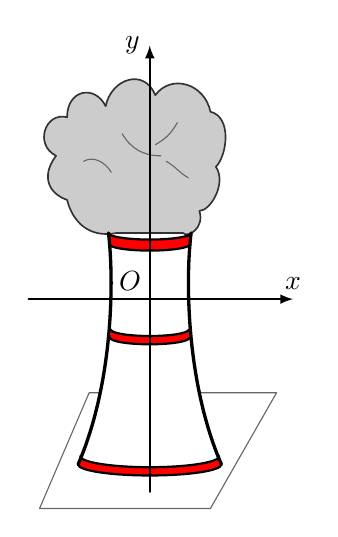
\begin{tikzpicture}[line join = round, line cap = round,>=stealth,scale=.7]
	% 1. Ground Plane (Parallelogram) - drawn behind the tower
	\draw[thin, color=gray!80!black] (-2.0, -3.8) -- (1.1, -3.8) -- (2.3, -1.7) -- (-1.1, -1.7) -- cycle;
	
	% 2. Smoke (Gray Cloud) - drawn behind the top of the tower
	\filldraw[fill=lightgray!80!white, draw=black!80, line width=0.6pt, line join=round]
	(-0.6, 1.2)
	.. controls (-1.1, 1.1) and (-1.4, 1.4) .. (-1.5, 1.8)
	.. controls (-1.8, 1.9) and (-2.0, 2.2) .. (-1.7, 2.6)
	.. controls (-2.1, 2.8) and (-1.9, 3.4) .. (-1.5, 3.3)
	.. controls (-1.5, 3.8) and (-1.0, 3.9) .. (-0.8, 3.5)
	.. controls (-0.7, 4.0) and (-0.1, 4.2) .. (0.1, 3.7)
	.. controls (0.4, 4.1) and (1.0, 3.9) .. (1.1, 3.4)
	.. controls (1.5, 3.3) and (1.4, 2.6) .. (1.2, 2.4)
	.. controls (1.4, 2.1) and (1.1, 1.6) .. (0.9, 1.6)
	.. controls (1.0, 1.3) and (0.7, 1.1) .. (0.6, 1.2)
	-- cycle;
	
	% Internal lines of the smoke cloud to give depth
	\draw[thin, color=black!60] (-1.2, 2.5) to[out=30, in=120] (-0.7, 2.3);
	\draw[thin, color=black!60] (-0.5, 3.0) to[out=-60, in=180] (0.2, 2.6);
	\draw[thin, color=black!60] (0.5, 3.2) to[out=-120, in=30] (0.1, 2.8);
	\draw[thin, color=black!60] (0.7, 2.2) to[out=150, in=-30] (0.3, 2.5);
	
	% 3. Tower Body (White Fill) - masks the ground plane and smoke base
	\fill[white] (-0.75, 1.2)
	.. controls (-0.65, 0.4) and (-0.65, -1.5) .. (-1.3, -3.0)
	arc (180:360:1.3 and 0.2)
	.. controls (0.65, -1.5) and (0.65, 0.4) .. (0.75, 1.2)
	arc (360:180:0.75 and 0.12);
	
	% 4. Red Bands Fills
	% Top Band
	\fill[red] (-0.75, 1.2) arc (180:360:0.75 and 0.12) -- (0.74, 1.0) arc (360:180:0.74 and 0.12) -- cycle;
	% Middle Band
	\fill[red] (-0.71, -0.55) arc (180:360:0.71 and 0.12) -- (0.72, -0.7) arc (360:180:0.72 and 0.12) -- cycle;
	% Bottom Band
	\fill[red] (-1.26, -2.85) arc (180:360:1.26 and 0.2) -- (1.3, -3.0) arc (360:180:1.3 and 0.2) -- cycle;
	
	% 5. Tower Outlines and Ribs
	% Thick Left and Right Boundaries
	\draw[very thick, line cap=round] (-0.75, 1.2) .. controls (-0.65, 0.4) and (-0.65, -1.5) .. (-1.3, -3.0);
	\draw[very thick, line cap=round] (0.75, 1.2) .. controls (0.65, 0.4) and (0.65, -1.5) .. (1.3, -3.0);
	
	% Front Elliptical Arcs of the Bands
	\draw[thick] (-0.75, 1.2) arc (180:360:0.75 and 0.12);
	\draw[thick] (-0.74, 1.0) arc (180:360:0.74 and 0.12);
	
	\draw[thick] (-0.71, -0.55) arc (180:360:0.71 and 0.12);
	\draw[thick] (-0.72, -0.7) arc (180:360:0.72 and 0.12);
	
	\draw[thick] (-1.26, -2.85) arc (180:360:1.26 and 0.2);
	\draw[thick] (-1.3, -3.0) arc (180:360:1.3 and 0.2);
	
	% 6. Coordinate Axes (drawn on top of the tower)
	% x-axis
	\draw[-latex, line width=0.6pt] (-2.2, 0) -- (2.6, 0) node[above] {$x$};
	% y-axis
	\draw[-latex, line width=0.6pt] (0, -3.5) -- (0, 4.6) node[left] {$y$};
	
	% 7. Labels
	\node[above left, inner sep=3pt] at (0,0) {$O$};
\end{tikzpicture}
}
	\loigiai{
		a) Đáy dưới của tháp là hình tròn có bán kính $R = 40\text{ m}$.\\
		Diện tích đáy dưới là: $S = \pi \cdot R^2 = \pi \cdot 40^2 = 1600\pi \approx 5027\text{ m}^2$.\\
		Do đó mệnh đề a) Đúng.\\
		b) Đoạn giao nhau giữa trục $Ox$ và tháp có độ dài bằng $30\text{ m}$.\\
		Vì trục $Oy$ là trục đối xứng nên hai giao điểm của $(H)$ với trục $Ox$ có tọa độ là $\left(-15; 0\right)$ và $\left(15; 0\right)$.\\
		Do đó các điểm $\left(-20; 0\right)$, $\left(20; 0\right)$ không thuộc hypebol $(H)$. Mệnh đề b) Sai.\\
		c) Phương trình chính tắc của hypebol $(H)$ có dạng $\dfrac{x^2}{a^2} - \dfrac{y^2}{b^2} = 1$.\\
		Vì $(H)$ cắt trục $Ox$ tại điểm $\left(15; 0\right)$ nên ta có $a = 15$.\\
		Mặt khác, tại độ cao đáy dưới $y = -80\text{ m}$ (vì gốc $O$ ở độ cao $80\text{ m}$ so với mặt đất), bán kính đáy là $x = 40\text{ m}$.\\
		Thay tọa độ điểm $\left(40; -80\right)$ thuộc $(H)$ vào phương trình ta được: \\
		$\dfrac{40^2}{15^2} - \dfrac{(-80)^2}{b^2} = 1 \Leftrightarrow  \dfrac{6400}{b^2} = \dfrac{1600}{225} - 1 = \dfrac{55}{9} \iff b^2 = \dfrac{11520}{11}$.\\
		Vậy phương trình của $(H)$ là $\dfrac{x^2}{15^2} - \dfrac{11y^2}{11520} = 1$.\\
		Do đó mệnh đề c) Sai.\\
		d) Thể tích của tháp giải nhiệt là thể tích khối tròn xoay được tạo ra khi quay hình phẳng giới hạn bởi đường hypebol $x = 15\sqrt{1 + \dfrac{11y^2}{11520}}$ quanh trục $Oy$ từ $y = -80$ đến $y = 40$ (đỉnh tháp cách gốc $O$ một khoảng là $120 - 80 = 40\text{ m}$):\\
		$V = \pi \displaystyle\int\limits_{-80}^{40} x^2 \mathrm{\,d}y = \pi \displaystyle\int\limits_{-80}^{40} 15^2 \left( 1 + \dfrac{11y^2}{11520} \right) \mathrm{\,d}y = \pi \displaystyle\int\limits_{-80}^{40} \left( 225 + \dfrac{55}{256}y^2 \right) \mathrm{\,d}y$\\
		$V = \pi \left.\left( 225y + \dfrac{55}{768}y^3 \right)\right|_{-80}^{40} = 68250\pi \approx 214414\text{ m}^3$.\\
		Do đó mệnh đề d) Đúng.
	}
\end{ex}
\begin{ex}
	
	Bạn Bắc chuẩn bị đi dã ngoại tại Bùi Hui trong hai ngày thứ Bảy và Chủ nhật. Biết rằng ở Bùi Hui, mỗi ngày chỉ có nắng hoặc mưa, nếu một ngày là nắng thì khả năng ngày hôm sau vẫn nắng là $80\%$, còn nếu một ngày là mưa thì khả năng ngày hôm sau vẫn mưa là $30\%$. Theo dự báo thời tiết, xác suất trời sẽ nắng vào thứ Bảy là $70\%$.
	
	\choiceTF
	{\True Xác suất để cả hai ngày nắng là $0{,}56$.}
	{Xác suất để có ít nhất một ngày nắng là $0{,}9$.}
	{\True Xác suất để Chủ nhật nắng là $0{,}77$.}
	{Biết Chủ nhật là ngày nắng, xác suất để thứ Bảy là ngày nắng là $0{,}7$.}
	
	\loigiai{
		
		Gọi:
		\begin{itemize}
			\item $A$: ``Trời nắng vào thứ Bảy''.
			\item $B$: ``Trời nắng vào Chủ nhật''.
		\end{itemize}
		
		Theo đề bài:
		$
		P(A)=0,7,\qquad P(\overline{A})=0,3.
		$
		
		Nếu thứ Bảy nắng thì khả năng Chủ nhật tiếp tục nắng là $80\%$, nên
		$
		P(B|A)=0,8.
		$
		
		Nếu thứ Bảy mưa thì khả năng Chủ nhật tiếp tục mưa là $30\%$, do đó
		$
		P(B|\overline{A})=1-0,3=0,7.
		$
		
		\begin{itemize}
			\item Xác suất để cả hai ngày đều nắng:
			$
			P(A\cap B)=P(A)\cdot P(B|A)
			$
			$
			=0,7\cdot 0,8=0,56.
			$
			
			Vậy khẳng định thứ nhất đúng.
			
			\item Xác suất để có ít nhất một ngày nắng:
			
			Biến cố đối là cả hai ngày đều mưa:
			$
			P(\overline{A}\cap \overline{B})
			=0,3\cdot 0,3=0,09.
			$
			
			Do đó
			$
			P(A\cup B)
			=1-0,09=0,91.
			$
			
			Vậy khẳng định thứ hai sai.
			
			\item Xác suất để Chủ nhật nắng:
			
			Theo công thức xác suất toàn phần:
			$
			P(B)
			=P(B|A)P(A)+P(B|\overline{A})P(\overline{A})
			=0,8\cdot 0,7+0,7\cdot 0,3=0,77.
			$
			
			Vậy khẳng định thứ ba đúng.
			
			\item Theo công thức Bayes:
			$
			P(A|B)
			=
			\dfrac{P(A\cap B)}{P(B)}
			=		\dfrac{0,56}{0,77}
			\approx 0,727.
			$
			
			Không bằng $0,7$, nên khẳng định thứ tư sai.
		\end{itemize}
	}
\end{ex}

\Closesolutionfile{ans}
%P3
{\bf PHẦN III. Câu trắc nghiệm trả lời ngắn.}
\setcounter{ex}{0}
\Opensolutionfile{ans}[ans/18-26-2-QuangNgai-ChuyenLeKhiet-L2-KQ]
\begin{ex}
	Hai đội tuyển $A$ và $B$ tham gia giải bóng bàn. Mỗi đội có $7$ người đã được sắp xếp theo một thứ tự nhất định. Đầu tiên, người thứ nhất của đội $A$ đấu với người thứ nhất của đội $B$ và người thua sẽ bị loại. Sau đó, người chiến thắng đấu tiếp với người thứ hai của đội kia, các trận thi đấu tiếp theo diễn ra tương tự. Cuộc thi đấu kết thúc cho đến khi tất cả người chơi của $1$ đội đều bị loại và đội còn lại là chiến thắng. Hỏi có bao nhiêu cách diễn ra cuộc thi đấu?
	\shortans{3432}
	\loigiai{
		Giả sử cuộc thi đấu kết thúc và đội $A$ giành chiến thắng chung cuộc. Khi đó, toàn bộ $7$ vận động viên của đội $B$ đều đã bị loại, và đội $A$ có $k$ vận động viên bị loại với $0 \le k \le 6$.\\
		Tổng số trận đấu diễn ra là $7 + k$ trận. Trận đấu cuối cùng phải là trận thua của vận động viên thứ $7$ của đội $B$ trước một vận động viên của đội $A$.\\
		Trong $6 + k$ trận trước đó, có đúng $k$ trận mà vận động viên của đội $A$ thua. Số cách chọn $k$ trận thua này từ $6 + k$ trận là $C_{6+k}^{k}$ cách.\\
		Do đó, số cách diễn ra cuộc thi mà đội $A$ thắng là:\\
		$C_6^0 + C_7^1 + C_8^2 + C_9^3 + C_{10}^4 + C_{11}^5 + C_{12}^6 = 1716$ cách.\\
		Tương tự, số cách diễn ra cuộc thi mà đội $B$ thắng cũng là $1716$ cách.\\
		Vậy tổng số cách diễn ra cuộc thi đấu là:\\
		$1716 + 1716 = 3432$ cách.
	}
\end{ex}

\begin{ex}
	Hàm lượng các chất vitamin A, vitamin B và vitamin K chứa trong $100\text{ g}$ mỗi loại thực phẩm $X$ và $Y$ được cho bảng sau:
	\begin{center}
		\begin{tabular}{|c|c|c|c|}
			\hline
			& vitamin A (mg) & vitamin B (mg) & vitamin K (mg) \\ \hline
			$X$ & 200 & 600 & 8 \\ \hline
			$Y$ & 500 & 300 & 6 \\ \hline
		\end{tabular}
	\end{center}
	Từ hai loại thực phẩm $X$ và $Y$, người ta muốn tạo ra một lượng thực phẩm hỗn hợp chứa ít nhất $2\,000\text{ mg}$ vitamin A, $3\,000\text{ mg}$ vitamin B, $48\text{ mg}$ vitamin K. Lượng thực phẩm hỗn hợp có khối lượng nhỏ nhất thỏa mãn yêu cầu trên là bao nhiêu? (đơn vị: kilôgam; làm tròn đến hàng phần trăm)
	\shortans{0{,}66\text{ kg}}
	\loigiai{
		\begin{center}
			\begin{tikzpicture}[line join=round, line cap=round, >=stealth,font=\footnotesize, scale=0.6]
				\draw[->](-2,0)--(12,0) node[below right] {$x$};
				\draw[->](0,-1)--(0,11) node[above] {$y$};
				\node (0,0) [below left]{$ O $};
				\foreach \x in {-1,...,2}
				\draw[shift={(\x,0)},color=black] (0pt,2pt) -- (0pt,-2pt);
				\foreach \y in {1,...,3}
				\draw[shift={(0,\y)},color=black] (2pt,0pt) -- (-2pt,0pt);
				\draw[samples=100,smooth,domain=-0.333:5.5] plot(\x,{-2*(\x)+10});
				\draw[samples=100,smooth,domain=-1:11] plot(\x,{-0.4*(\x)+4});
				\draw[samples=100,smooth,domain=-1:6.5] plot(\x,{-4/3*(\x)+8});
				\fill[pattern=crosshatch dots] (-1.3,-1)--(0,-1)--(0,11.1)--(-1.3,11.1)--cycle;
				\fill[pattern=crosshatch dots] (-1.3,-1.3)--(11.3,-1.3)--(11.3,0)--(-1.3,0)--cycle;
				\fill[pattern=crosshatch dots] (-1,22/5)--(12,-4/5)--(12,-1.3)--(-1,-1.3)--cycle;
				\fill[pattern=crosshatch dots] (-0.5,11)--(5.5,-1)--(5.5,-1.3)--(-1,4)--cycle;
				\fill[pattern=crosshatch dots] (-1,28/3)--(6.5,-2/3)--(6.5,-1.3)--(-1,4)--cycle;
				\node[above right] at (10,0) {$D$};
				\node[above right] at (0,10) {$C$};
				\node[right] at (3,4) {$B$};
				\node[right] at (30/7,16/7) {$A$};
				\node[above right,rotate=-28] at (7,1.5) {$2x+5y=20$};
				\node[above right,rotate=-70] at (1,10) {$2x+y=10$};
				\node[above right,rotate=-60] at (1,5.5) {$4x+3y=24$};
				
			\end{tikzpicture}
		\end{center}
		Gọi $x$ và $y$ lần lượt là số lần lượng thực phẩm $100\text{ g}$ của loại $X$ và loại $Y$ được sử dụng ($x \ge 0, y \ge 0$).\\
		Khi đó, khối lượng của hỗn hợp thực phẩm là:\\
		$m = 100x + 100y\text{ (g)} = 0{,}1x + 0{,}1y\text{ (kg)}$.\\
		Để tìm khối lượng nhỏ nhất, ta cần tìm giá trị nhỏ nhất của biểu thức $F(x, y) = x + y$.\\
		Từ giả thiết bài toán, ta có hệ bất phương trình ràng buộc sau:\\
		$$\begin{cases} 200x + 500y \ge 2000 \\ 600x + 300y \ge 3000 \\ 8x + 6y \ge 48 \\ x \ge 0 \\ y \ge 0 \end{cases} \Leftrightarrow \begin{cases} 2x + 5y \ge 20 \quad (1) \\ 2x + y \ge 10 \quad (2) \\ 4x + 3y \ge 24 \quad (3) \\ x \ge 0 \\ y \ge 0. \end{cases}$$Biểu diễn miền nghiệm của hệ bất phương trình trên mặt phẳng tọa độ $Oxy$, miền nghiệm là miền không bị giới hạn có các đỉnh là:\\
		$C\left(0; 10\right)$ là giao điểm của đường thẳng $2x + y = 10$ với trục $Oy$.\\
		$B\left(3; 4\right)$ là giao điểm của hai đường thẳng $2x + y = 10$ và $4x + 3y = 24$.\\
		$A\left(\dfrac{30}{7}; \dfrac{16}{7}\right)$ là giao điểm của hai đường thẳng $4x + 3y = 24$ và $2x + 5y = 20$.\\
		$D\left(10; 0\right)$ là giao điểm của đường thẳng $2x + 5y = 20$ với trục $Ox$.\\
		Tính giá trị của biểu thức $F(x, y) = x + y$ tại các đỉnh của miền nghiệm:\\
		Tại $C\left(0; 10\right)$: $F(0, 10) = 10$.\\
		Tại $B\left(3; 4\right)$: $F(3, 4) = 7$.\\
		Tại $A\left(\dfrac{30}{7}; \dfrac{16}{7}\right)$: $F\left(\dfrac{30}{7}, \dfrac{16}{7}\right) = \dfrac{46}{7} \approx 6{,}57$.\\
		Tại $D\left(10; 0\right)$: $F(10, 0) = 10$.\\
		Suy ra giá trị nhỏ nhất của $F(x, y)$ là $\dfrac{46}{7}$ đạt được tại $x = \dfrac{30}{7}$ và $y = \dfrac{16}{7}$.\\
		Khối lượng nhỏ nhất của hỗn hợp thực phẩm là:\\
		$m_{\min} = 0{,}1 \times \dfrac{46}{7} = \dfrac{46}{70} \approx 0{,}66\text{ kg}$.
	}
\end{ex}

\begin{ex}
	Một công ty du lịch thông báo giá tiền cho chuyến đi tham quan của một nhóm khách du lịch như sau: $20$ khách đầu tiên có giá là $30\text{ USD/người}$; nếu có nhiều hơn $20$ người đăng kí thì cứ có thêm $1$ người, giá vé sẽ giảm $1\text{ USD/người}$ cho toàn bộ hành khách. Hỏi công ty nên giới hạn số lượng hành khách tối đa là bao nhiêu để công ty không bị lỗ? Biết rằng chi phí của chuyến đi là $400\text{ USD}$.
	\shortans{40}
	\loigiai{
		Gọi $x$ là số lượng hành khách tham gia chuyến đi ($x \in \mathbb{N}^*$).\\
		Nếu $x \le 20$, tổng doanh thu của công ty là $30x\text{ USD}$.\\
		Để không bị lỗ thì $30x \ge 400 \Leftrightarrow x \ge 13{,}33$. Do đó nhóm khách phải từ $14$ đến $20$ người.\\
		Nếu $x > 20$, số lượng khách vượt quá $20$ người là $x - 20$.\\
		Khi đó, giá vé của mỗi người được giảm đi $(x - 20) \times 1 = x - 20\text{ USD}$.\\
		Giá vé cho mỗi hành khách lúc này là $30 - (x - 20) = 50 - x\text{ USD}$ (với điều kiện $x < 50$).\\
		Tổng doanh thu thu được từ chuyến đi là:\\
		$T(x) = x(50 - x) = 50x - x^2\text{ USD}$.\\
		Để công ty không bị lỗ thì doanh thu phải lớn hơn hoặc bằng chi phí chuyến đi:\\
		$50x - x^2 \ge 400 \Leftrightarrow x^2 - 50x + 400 \le 0 \Leftrightarrow 10 \le x \le 40$.\\
		Kết hợp với điều kiện $x > 20$, ta được $20 < x \le 40$.\\
		Do đó, để đảm bảo không bị lỗ khi số lượng khách đăng ký lớn hơn $20$ người, số lượng hành khách tối đa không vượt quá $40$ người.\\
		Vậy công ty nên giới hạn số lượng hành khách tối đa là $40$ người.
	}
\end{ex}

\begin{ex}
	\immini{
	Một viên gạch hình vuông $ABCD$ có cạnh $60$. Người ta trang trí viên gạch bằng các đường cong $(L_1), (L_2)$. $(L_1)$ là tập hợp các điểm $M$ thỏa $MC = MA + 50$ hoặc $MA = MC + 50$. Khi quay đường cong $(L_1)$ quanh tâm viên gạch hình vuông đó một góc $90^\circ$ ta được đường cong $(L_2)$. Tính diện tích hình phẳng giới hạn bởi các đường cong $(L_1), (L_2)$ và các cạnh viên gạch (phần màu trắng, kết quả làm tròn đến hàng đơn vị).
	}{
		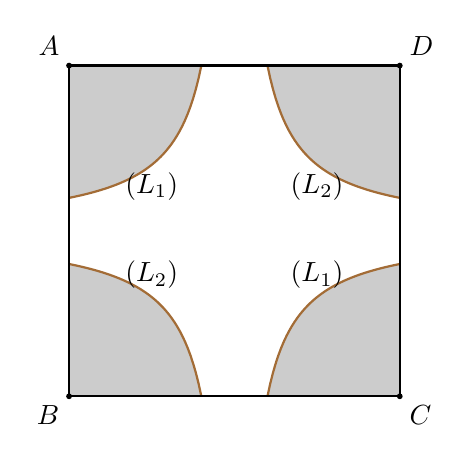
\begin{tikzpicture}[scale=0.7]
			% Coordinates of the vertices
			\coordinate (A) at (0,6);
			\coordinate (B) at (0,0);
			\coordinate (C) at (6,0);
			\coordinate (D) at (6,6);
			
			% Fill the shaded corner regions using hyperbola branches
			% Domain is set carefully for each corner to draw the curve smoothly
			\fill[gray!40] (A) -- (0, 3.6) -- plot[domain=0:2.4, samples=50] (\x, {3 - 1.8/(\x-3)}) -- cycle;
			\fill[gray!40] (B) -- (0, 2.4) -- plot[domain=0:2.4, samples=50] (\x, {3 + 1.8/(\x-3)}) -- cycle;
			\fill[gray!40] (C) -- (3.6, 0) -- plot[domain=3.6:6, samples=50] (\x, {3 + 1.8/(3-\x)}) -- cycle;
			\fill[gray!40] (D) -- (3.6, 6) -- plot[domain=3.6:6, samples=50] (\x, {3 - 1.8/(3-\x)}) -- cycle;
			
			% Draw the curved hyperbola boundaries in brown
			\draw[brown!85!black, thick] plot[domain=0:2.4, samples=50] (\x, {3 - 1.8/(\x-3)});
			\draw[brown!85!black, thick] plot[domain=0:2.4, samples=50] (\x, {3 + 1.8/(\x-3)});
			\draw[brown!85!black, thick] plot[domain=3.6:6, samples=50] (\x, {3 + 1.8/(3-\x)});
			\draw[brown!85!black, thick] plot[domain=3.6:6, samples=50] (\x, {3 - 1.8/(3-\x)});
			
			% Draw the square border
			\draw[thick] (B) rectangle (D);
			
			% Draw the vertices and their labels
			\fill (A) circle (1.5pt) node[above left] {$A$};
			\fill (B) circle (1.5pt) node[below left] {$B$};
			\fill (C) circle (1.5pt) node[below right] {$C$};
			\fill (D) circle (1.5pt) node[above right] {$D$};
			
			% Labels for the curves
			\node at (1.5, 3.8) {$(L_1)$};
			\node at (4.5, 3.8) {$(L_2)$};
			\node at (1.5, 2.2) {$(L_2)$};
			\node at (4.5, 2.2) {$(L_1)$};
		\end{tikzpicture}
	}
	\shortans{2502}
	
	\loigiai{
		Chọn hệ trục tọa độ sao cho tâm của hình vuông là gốc tọa độ $O(0;0)$.\\
		Thực hiện phép quay hệ trục một góc phù hợp sao cho hai tiêu điểm của đường cong $(L_1)$ nằm trên trục hoành. Do $ABCD$ là hình vuông cạnh $60$, hai tiêu điểm là $A$ và $C$ có khoảng cách là $AC = 60\sqrt{2}$.\\
		Khi đó, đường cong $(L_1)$ là một hyperbol có phương trình:
		\[\dfrac{x^2}{a^2} - \dfrac{y^2}{b^2} = 1\]
		Với $2a = 50 \implies a = 25$ và $c = 30\sqrt{2} \implies b^2 = c^2 - a^2 = (30\sqrt{2})^2 - 25^2 = 1175$.\\
		Vậy phương trình của $(L_1)$ là:
		\[\dfrac{x^2}{625} - \dfrac{y^2}{1175} = 1\]
		Đường cong $(L_2)$ thu được bằng cách xoay $(L_1)$ một góc $90^\circ$, có phương trình:
		\[\dfrac{y^2}{625} - \dfrac{x^2}{1175} = 1\]
		Xét nhánh phía trên của $(L_2)$ gần đỉnh $D(0; 30\sqrt{2})$ có phương trình:
		\[y = 25\sqrt{1 + \dfrac{x^2}{1175}}\]
		Hai cạnh của hình vuông đi qua $D$ có phương trình lần lượt là $y = x + 30\sqrt{2}$ và $y = -x + 30\sqrt{2}$.\\
		Hoành độ giao điểm của nhánh $(L_2)$ này với đường thẳng $y = x + 30\sqrt{2}$ (với $x < 0$) là nghiệm của phương trình:
		\[25\sqrt{1 + \dfrac{x^2}{1175}} = x + 30\sqrt{2} \implies x_0 \approx -15{,}11\]
		Diện tích phần màu xám ở góc $D$ là:
		\[S_1 = \displaystyle\int\limits_{x_0}^{-x_0} \left( -|x| + 30\sqrt{2} - 25\sqrt{1 + \dfrac{x^2}{1175}} \right) \mathrm{\,d}x \approx 274{,}5\]
		Do tính đối xứng, diện tích của 4 phần màu xám ở 4 góc là:
		\[S_{\text{xám}} = 4 \times S_1 \approx 1098\]
		Diện tích phần màu trắng cần tìm là:
		\[S = S_{ABCD} - S_{\text{xám}} = 60^2 - 1098 = 2502\]
	}
\end{ex}

\begin{ex}
	Cho hình lăng trụ tam giác đều $ABC.A'B'C'$ có tất cả các cạnh bằng $2\text{ cm}$. Gọi $M$ và $N$ lần lượt là trung điểm $B'C'$ và $A'B'$. Gọi $\alpha$ là góc tạo bởi $MN$ và $(BCC'B')$. Tính $\tan^2 \alpha$.
	\shortans{3}
	\loigiai{
		Gọi $H$ là trung điểm của $B'M$. Do $M$ là trung điểm của $B'C'$ nên $B'M = 1\text{ cm}$ và $MH = \dfrac{1}{2}\text{ cm}$.\\
		Trong tam giác đều $A'B'C'$, đường trung tuyến $A'M$ đồng thời là đường cao nên $A'M \perp B'C'$.\\
		Vì $N$ là trung điểm của $A'B'$ và $H$ là trung điểm của $B'M$ nên $NH \parallel A'M$ và $NH = \dfrac{1}{2} A'M$.\\
		Độ dài đường cao trong tam giác đều cạnh $2$ là $A'M = \sqrt{3}\text{ cm}$, suy ra $NH = \dfrac{\sqrt{3}}{2}\text{ cm}$.\\
		Do lăng trụ tam giác đều nên mặt bên $(BCC'B') \perp (A'B'C')$. Vì $NH \perp B'C'$ (do $NH \parallel A'M$ và $A'M \perp B'C'$) nên $NH \perp (BCC'B')$.\\
		Khi đó, hình chiếu vuông góc của $N$ trên mặt phẳng $(BCC'B')$ là $H$.\\
		Điểm $M \in B'C'$ nên hình chiếu của $M$ trên $(BCC'B')$ chính là $M$.\\
		Suy ra góc giữa đường thẳng $MN$ và mặt phẳng $(BCC'B')$ là góc giữa hai đường thẳng $MN$ và $MH$, chính là góc $\alpha = \widehat{NMH}$.\\
		Tam giác $MHN$ vuông tại $H$, ta có:
		\[\tan \alpha = \dfrac{NH}{MH} = \dfrac{\dfrac{\sqrt{3}}{2}}{\dfrac{1}{2}} = \sqrt{3}\]
		Vậy $\tan^2 \alpha = 3$.
	}
\end{ex}

\begin{ex}
	Bốn tay vợt Tennis An, Bình, Công và Duy tham gia vào một giải đấu có tổng cộng ba trận đấu. Đầu tiên, hai người chơi được chọn ngẫu nhiên để chơi với nhau; hai người chơi còn lại cũng chơi với nhau. Những người chiến thắng trong hai trận đấu đó sẽ thi đấu với nhau để quyết định nhà vô địch giải đấu. An, Bình và Công ngang sức nhau (nghĩa là, khi một trận đấu được chơi giữa hai người trong ba người An, Bình, Công, xác suất mỗi người chơi thắng là $\dfrac{1}{2}$). Khi Duy đấu với An, Bình hoặc Công, xác suất Duy thắng là $0.7$. Xác định xác suất Bình vô địch giải đấu.
	\shortans{0.17}
	\loigiai{
		Kí hiệu các đấu thủ là $A$ (An), $B$ (Bình), $C$ (Công), $D$ (Duy).\\
		Có 3 trường hợp chia cặp đấu đầu tiên xảy ra với xác suất bằng nhau và bằng $\dfrac{1}{3}$:\\
		\textbf{Trường hợp 1:} Cặp đấu đầu tiên là $\{A, B\}$ và $\{C, D\}$.\\
		- Để $B$ vô địch, trước hết $B$ phải thắng $A$ (xác suất $0.5$).\\
		- Trận đấu còn lại giữa $C$ và $D$ có kết quả:\\
		+ $C$ thắng $D$ với xác suất $0.3$. Khi đó chung kết là $B$ gặp $C$, $B$ thắng với xác suất $0.5$.\\
		+ $D$ thắng $C$ with xác suất $0.7$. Khi đó chung kết là $B$ gặp $D$, $B$ thắng với xác suất $1 - 0.7 = 0.3$.\\
		- Xác suất $B$ vô địch trong trường hợp này là:
		\[P_1 = 0.5 \times (0.3 \times 0.5 + 0.7 \times 0.3) = 0.5 \times (0.15 + 0.21) = 0.18\]
		\textbf{Trường hợp 2:} Cặp đấu đầu tiên là $\{A, C\}$ và $\{B, D\}$.\\
		- Để $B$ vô địch, trước hết $B$ phải thắng $D$ (xác suất $0.3$).\\
		- Trận đấu còn lại giữa $A$ và $C$ có kết quả:\\
		+ $A$ thắng $C$ với xác suất $0.5$. Chung kết $B$ gặp $A$, $B$ thắng với xác suất $0.5$.\\
		+ $C$ thắng $A$ với xác suất $0.5$. Chung kết $B$ gặp $C$, $B$ thắng với xác suất $0.5$.\\
		- Xác suất $B$ vô địch trong trường hợp này là:
		\[P_2 = 0.3 \times (0.5 \times 0.5 + 0.5 \times 0.5) = 0.3 \times 0.5 = 0.15\]
		\textbf{Trường hợp 3:} Cặp đấu đầu tiên là $\{A, D\}$ và $\{B, C\}$.\\
		Do vai trò của $A$ và $C$ đối với $B$ và $D$ hoàn toàn đối xứng, trường hợp này có xác suất $B$ vô địch tương tự như Trường hợp 1:\\
		\[P_3 = 0.18\]
		Xác suất tổng hợp để Bình vô địch giải đấu là:
		\[P = \dfrac{1}{3} P_1 + \dfrac{1}{3} P_2 + \dfrac{1}{3} P_3 = \dfrac{1}{3} (0.18 + 0.15 + 0.18) = \dfrac{0.51}{3} = 0.17\]
	}
\end{ex}

\Closesolutionfile{ans}
